\documentclass[titlepage,a4paper]{jsarticle}
\usepackage{../../sty/import}% 各種パッケージインポート
\usepackage{../../sty/B4_reserch}% タイトルページの変更

%% タイトルページの変数
% レポートタイトル
\midpapertitle{大規模言語モデルと動画生成AIを組み合わせた英語学習システムの構築}
\studentid{24336488}
\studentname{本間 三暉}
\supervisor{湯川 高志}
%
\begin{document}
% titleページ作成
\maketitle
\section{研究背景・目的}
昨今,国際的な技術力の競争が激化しており,技術者には英語論文や技術書を読み,知見を共有する力が不可欠である.
しかし工学系大学生には英語への苦手意識が強く,単語帳学習など従来手法ではモチベーション維持と定着が難しい.
そこで,本研究ではエピソード記憶理論と二段階の AI 活用に基づく学習支援システムを提案する.

\section{個別最適化システム}
提案するシステムは,エピソード記憶理論\cite{epi}に基づき,AIが学習者一人ひとりに最適化した動画を自動生成する英語学習システムで,
AIを用いて学習者の興味に近い文脈の中で単語を視覚的に学習することで記憶への定着を促す.
\begin{figure}[H]
    \centering
    % 左側の画像
    \begin{minipage}[t]{0.2\textwidth}
        \centering
        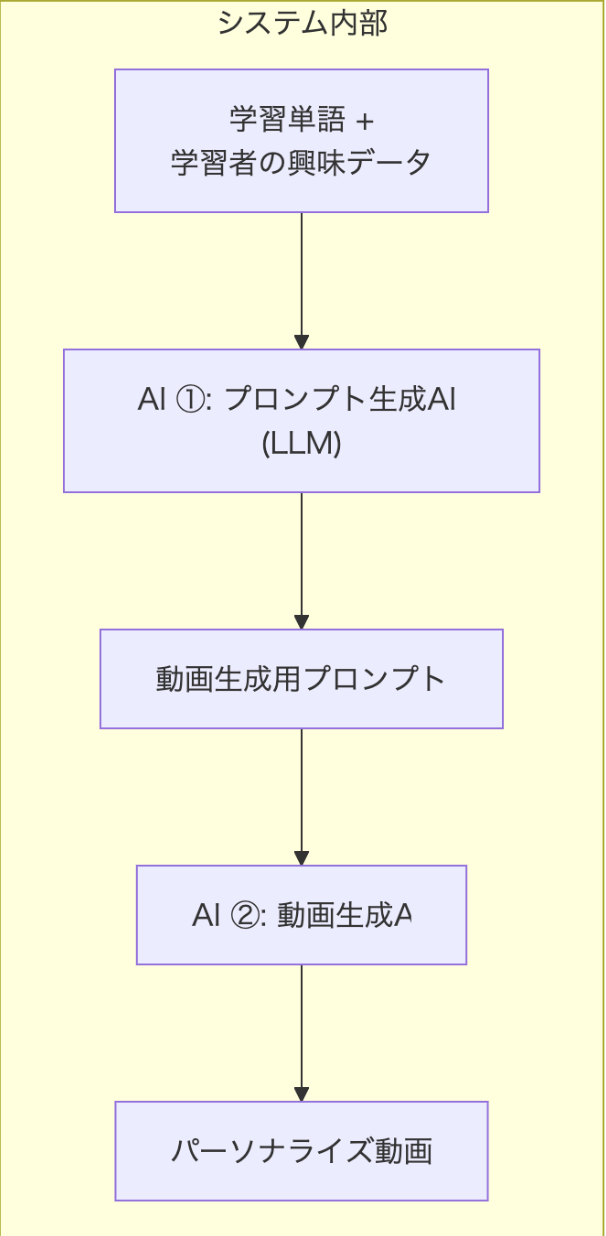
\includegraphics[width=\textwidth]{img/sysin.png}
        \caption{動画生成システム内部のフローチャート}
        \label{system_in}
    \end{minipage}
    \hfill % 隙間を作る
    % 右側の画像
    \begin{minipage}[t]{0.2\textwidth}
        \centering
        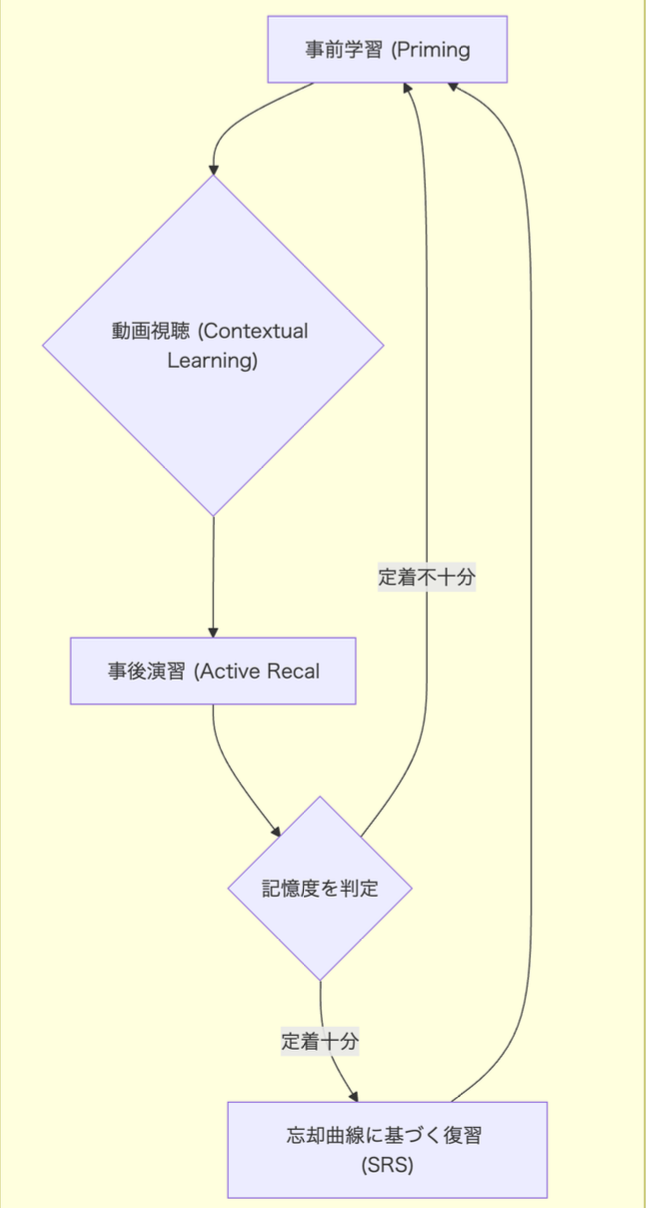
\includegraphics[width=\textwidth]{img/sysout.png}
        \caption{システムを用いた学習サイクル}
        \label{system_out}
    \end{minipage}
\end{figure}
このシステムのフローチャートを図\ref{system_in}に示す.
まず,アンケートなどから得た学習者の興味データと覚えたい任意の英単語からLLMが動画のシナリオ(プロンプト)を背景情報も含めて考案する.
次にそのプロンプトを元に動画生成AIが映像を作成する.
これにより,学習者の学習意欲を刺激する個別最適化された教材が実現する.

また,システムを用いた学習サイクルについて図\ref{system_out}に示す.
単語やその意味について知る事前学習,AIにより生成された動画を見る動画視聴,学習した単語が定着しているかを測る事後学習をサイクルさせることで,知識のインプットからアウトプットまでをサポートする.
これにより,ただ視聴するだけでなく,能動的な学習を促し,記憶の定着率を高めることが出来ると考える.

一つの単語に対し,AIが文脈の異なる複数の動画を生成し,それらを見比べることで単語の表面的なイメージではなく,根底にある共通のイメージを直感的に掴むことが出来る.

さらに,Spaced Repetition System(SRS)を導入し,学習データから忘れやすいタイミングを予測して復習問題を出題することによって,学習内容を長期記憶へと定着させることが出来ると考える.

\section{評価方法}
\subsection*{被験者}
長岡技術科学大学の学生
\subsection*{グループ分け}
TOEIC 事前テストで点数が均等になるよう,本システムを用いる\textbf{実験群}と従来学習で自習する\textbf{統制群}に分ける.

\subsection*{評価指標}
\begin{itemize}
  \item \textbf{定量評価}:TOEIC 前後差を t 検定で比較し学習効果を検証する.
  \item \textbf{定性評価}:アンケートとインタビューで学習意欲・満足度を調査する.
\end{itemize}
\section{今後の予定}
\begin{itemize}
  \item プロトタイプ実装→効果測定→分析・考察
\end{itemize}

% ------------------------------------------------------------

% 参考文献
\begin{thebibliography}{99}
\bibitem{epi}若原雅斗,松田結希,下里祐介,濱川礼:拡張現実を用いた次世代型英語学習システムの提案,第74回全国大会講演論文集,2012,1,pp.317-318,2012-03-06.
\url{https://ipsj.ixsq.nii.ac.jp/records/110507}
\bibitem{}吉田葵,青柳龍也,来住伸子:動画スクリプトを利用した多肢選択問題の自動生成,第52回プログラミング・シンポジウム予稿集,2011,pp.21-28,2011-01-07.
\url{https://ipsj.ixsq.nii.ac.jp/records/91419}
\end{thebibliography}

\end{document}